\section{Auto-Organização Emergente}

\subsection{Sistemas Auto-Organizáveis}

Organização é definida em~\cite{Heylighen2003} como estrutura com função. Um sistema pode ser chamado de \emph{organizado} se possuir uma certa estrutura e funcionalidade. Estrutura significa que os componentes são organizados em certa ordem. Função significa que o sistema tem que cumprir algum objetivo.

Um sistema é auto-organizado se ele é organizado sem nenhum controle externo ou central~\cite{Heylighen2003}. As entidades individuais interagem entre si localmente. Portanto,  auto-organização pode ser definida como um processo dinâmico e adaptativo onde o sistema adquire e mantém estruturas sem nenhum controle externo~\cite{DeWolf2005a}.

As seguintes características são empregadas para se descrever um sistema auto-organizável~\cite{DeWolf2005a}:
\begin{description}
 \item [Aumento da ordem:] Uma característica importante é a ``organização' do sistema. Partes selecionadas do sistema são arranjadas de forma a promover uma função específica. Isso restringe o comportamento do sistema a uma pequena parcela de todos os comportamentos possíveis.

Um aumento de ordem requer que o sistema inicie de um estado não-organizado ou semi-organizado, sem memória sobre o histórico do sistema. O aumento da organização requer um gradual aumento da memória deste histórico. Contudo, um sistema auto-organizável precisa manter um balanço entre a ordem e o excesso de ordem, pois o excesso da mesma acarretaria com que o sistema não produzisse nenhuma função específica.

\item[Autonomia:] Em um sistema auto-organizável, é muito importante a ausência de um controle externo. Para se determinar se o sistema é auto-organizável torna-se necessário o estabelecimento de limites quanto a autonomia de cada indivíduo.

\item[Adaptabilidade e Robustez:] Um sistema auto-organizável normalmente se adapta automaticamente quando o ambiente em que se encontra inserido sofre modificações. Essa adaptabilidade, consequentemente, promove um aumento na robustez do sistema.

%\item[Dinâmico ou longe do equilíbrio:]

\end{description}


\subsection{Sistemas Emergentes}

Um sistema é considerado emergente se propriedades, estruturas ou um padrão coerente emerge no nível macro que surgem em resposta às iterações entre as partes no nível micro. Essas estruturas não podem ser explicadas por uma simples combinação linear das partes individuais do sistema.

As seguintes características podem ser atribuídas a um sistema emergente~\cite{DeWolf2005a}:
\begin{description}

 \item [Efeito micro-macro:] Característica mais importante.%, citada extensivamente na literatura (\cite{olhar no paper}). 
Esse efeito se refere às estruturas que se situam em nível macro, estas, conseqüências das interações não lineares entre os componentes em nível micro do sistema.

 \item[Novidade radical:] O comportamento global do sistema é novo quando comparado ao comportamento individual dos componentes no nível micro do sistema. Utilizando reducionismo para a formulação, pode-se dizer que as estruturas no nível macro não são redutíveis aos componentes do nível micro. Isso significa que o sistema tem que ser estudado como um todo, não podendo ser entendido apenas avaliando-se um componente sem considerar o contexto no qual este se insere.

\item[Coerência:] Se refere a coerência lógica entre as partes do sistema. O padrão formado tende a manter uma identidade no tempo.

\item[Interação:] As partes básicas do sistema precisam interagir. Sem interação, o efeito micro-macro não surgirá.

\item[Controle descentralizado:] Somente controle local é usado para influenciar o comportamento global. Não existe uma unidade central responsável por coordenar o comportamento do sistema.

\item[Dinâmico:] Padrões emergentes aparecem com o desenvolvimento do sistema no tempo. Têm relação com aparecimento de atratores em sistemas dinâmicos.

\item[Ligação bidirecional:] Existe uma ligação bidirecional entre os níveis micro e macro do sistema. Do nível micro para o macro, as partes se organizam em padrões emergentes. Do nível macro para o micro, as estruturas emergentes influenciam as partes. Propriedades de alto nível podem causar efeitos no nível mais baixo.

\item[Robustez e flexibilidade:] O fato do controle ser descentralizado e não existir uma entidade única que tenha a representação emergente global implica que não existe ponto único de falha. Normalmente, padrões emergentes são insensíveis à perturbações e erros, apresentando uma degradação gradual quando componentes falham.

\end{description}


\subsection{Combinação entre Auto-Organização e Emergência}

Em um sistema complexo, distribuído, composto de um grande número de unidades, a auto-organização torna-se uma característica desejável, visto que um controle centralizado externo nem sempre é possível. Uma ordem crescente no sistema, que promova uma dada função é o objetivo que se quer alcançar com a auto-organização. 

Normalmente os indivíduos do sistema apresentam estruturas simples e não possuem autonomia para lidar diretamente a complexidade do sistema. Portanto, espera-se que um comportamento global coerente surja das interações desses elementos. 


Isto significa que um comportamento emergente é requerido do sistema. Assim, o comportamento emergente é responsável por guiar a organização do sistema no nível macro. Com a combinação  entre os dois conceitos apresentados, obtém-se a Auto-Organização Emergente.


Uma característica adicional que se pode encontrar em auto-organização emergente é:
\begin{description}
 \item [Não linearidade:] Um sistema onde a emergência é utilizada para a auto-organização pode requerer o princípio de "pequena causa/grande efeito" e apresentar um foco intenso em interações não-lineares.~\cite{DeWolf2005a}. Este efeito normalmente é modelado pelo modo de interação de realimentação positiva. Realimentação positiva normalmente produz mudança no sistema~\cite{Camazine2001}. O efeito de amplificação diretamente leva ao desenvolvimento de padrões no sistema~\cite{Dressler2007}%super livro SO WSN}. 
A realimentação positiva é também chamada de auto-catálise: um tipo de padrão causa o aumento do mesmo tipo, gerando um efeito bola de neve. Para controlar o efeito destrutivo da realimentação positiva e dar uma forma ao sistema utiliza-se realimentação negativa.

\end{description}

Na figura \ref{fig:conceps}, os possíveis tipos de sistemas são mostrados. 

%%nao consigo colocar essa figura direito.. está dando problema

\begin{figure}
 \centering
 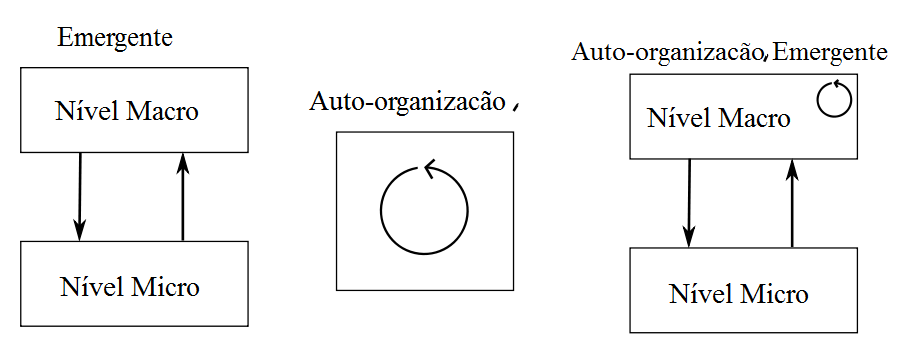
\includegraphics[width=10cm]{pictures/concepts.png}
 % concepts.eps: 1179666x1179666 pixel, 300dpi, 9987.84x9987.84 cm, bb=134 396 423 492
 \caption{Conceitos apresentados. (a) Sistema emergente. (b) Sistema auto-organizável. (c) Sistema auto-organizável emergente.}
 \label{fig:conceps}
\end{figure}


